
For example, a photon with an energy of the order of one MeV has a
mean free path of several centimeters in the germanium crystal. It
most probably deposits energy in several different segments because of
multiple Compton scattering. The result is a \emph{multi-segment
  event}, in short MSE. In contrast, if there is only one segment with
an energy deposition, it is called a \emph{single-segment event}, in
short SSE. The power of discrimination of MSE and SSE induced by
photon using segmented germanium detectors has been shown in
\cite{Pid07}.

\section{Monte Carlo simulation} 
\label{sec:ph:sim}
Monte Carlo simulations of prototype detectors and their cryostats was
performed using MaGe~\cite{Mag08}, a C++ package co-developed by the
Majorana and GERDA collaborations using Geant4
toolkits~\cite{Gea03,Gea06}. Figure~\ref{fig:ph:sim} shows the
geometry models of the detectors and cryostats implemented in Geant4.
The right plot of Fig~\ref{fig:ph:sim} shows a close-up of the
\emph{Siegfried} II geometry. It was modeled in such a way that the
details were implemented as close as possible to reality while the
simulation efficiency did not decrease too much.

The energy depositions of hits in each segment were recorded and the
core energy was calculated by adding all segment energies. The segment
and core energies were individually smeared according to the energy
resolutions of the detectors measured in the individual channels.

The spacial and time information of hits were also recorded, which
served as parts of the input for the pulse shape simulation package.
The geometry of detectors and the voltage bias applied were other
input information for the pulse shape simulation. The detail of the
pulse shape simulation is described in Chapter~\ref{cha:pss}.
 
\begin{figure}[tbhp]
  \centering
  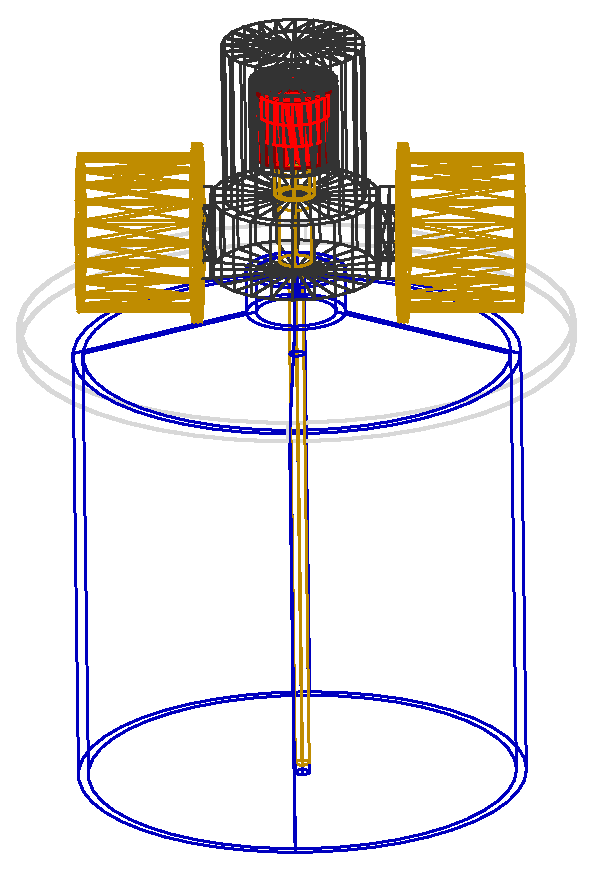
\includegraphics[height=0.3\textheight,clip]{SIwired}\hfil
  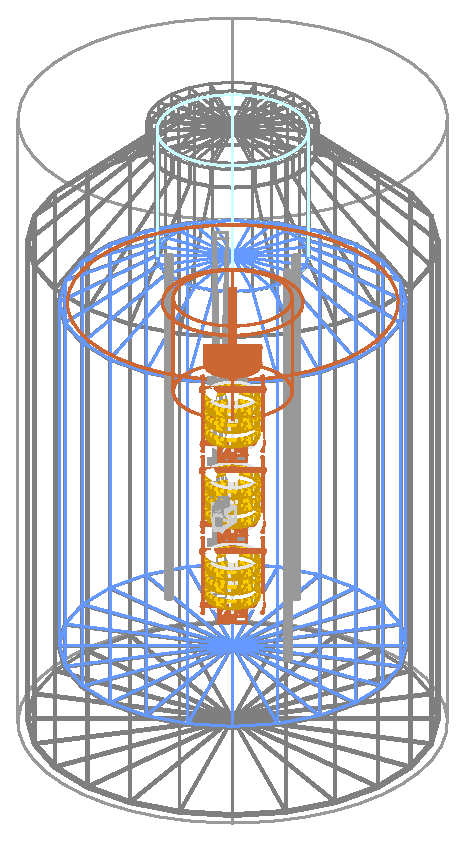
\includegraphics[height=0.3\textheight,clip]{GIIwired}\hfil
  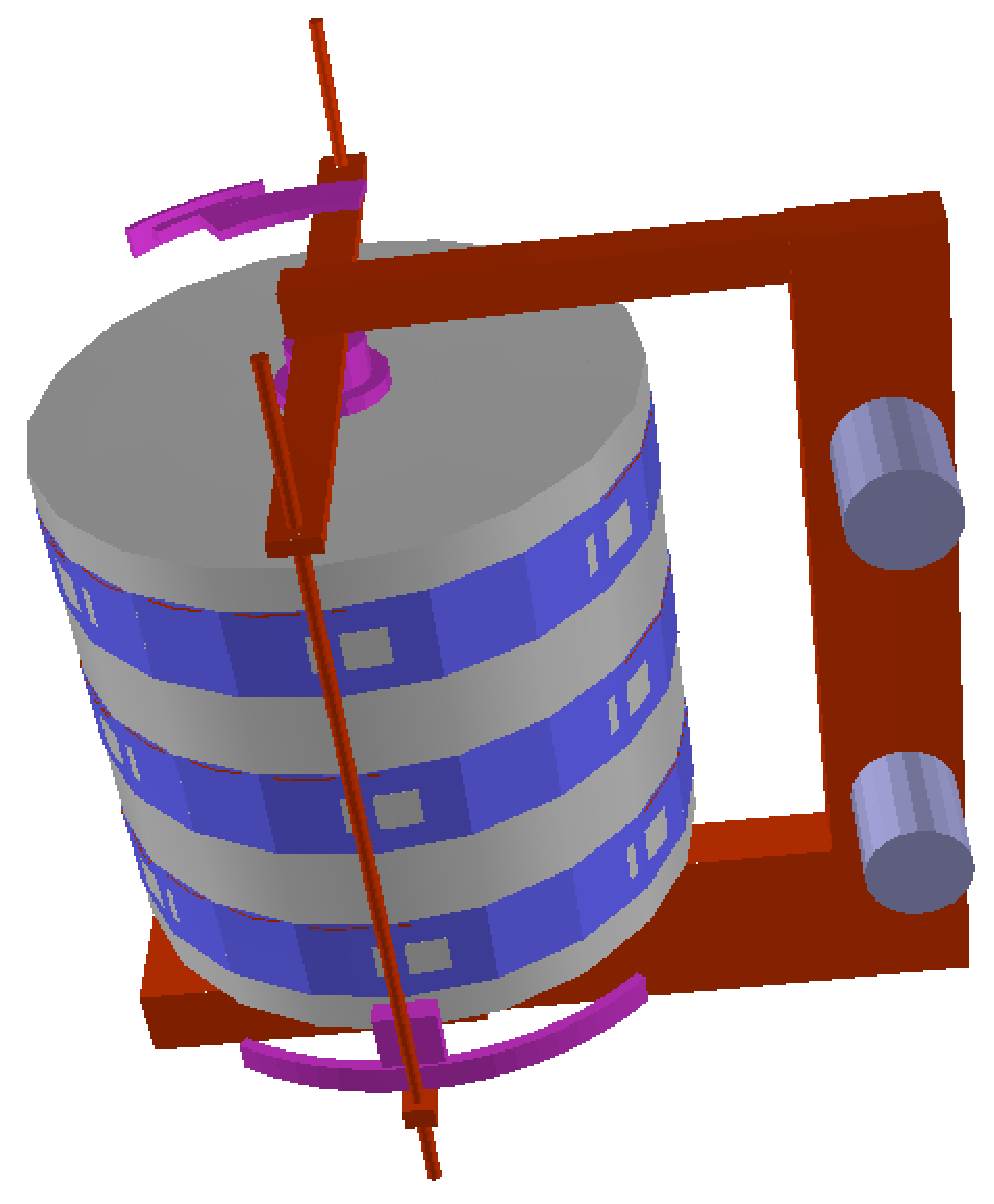
\includegraphics[height=0.3\textheight,clip]{SIIsolid}
  \caption{Left: wired drawing of the commercial cryostat geometry.    
Middle: wired drawing of Gerdalinchen II geometry. Right: a    
close-up of \emph{Siegfried} II geometry with copper supporting    
frame as used in Gerdalinchen II.}
  \label{fig:ph:sim}
\end{figure}



%%% Local Variables:
%%% mode:latex
%%% TeX-master: "thesis"
%%% End: